\documentclass[12pt]{report}
\usepackage[a4paper]{geometry}
\usepackage[utf8]{inputenc}
\usepackage[myheadings]{fullpage}
\usepackage{fancyhdr}
\usepackage{lastpage}
\usepackage{float}
\usepackage{graphicx, wrapfig, subcaption, setspace, booktabs}
\usepackage{graphicx}
\usepackage[T1]{fontenc}
\usepackage[font=small, labelfont=bf]{caption}
\usepackage{fourier}
\usepackage[protrusion=true, expansion=true]{microtype}
\usepackage[english]{babel}
\usepackage{sectsty}
\usepackage{url, lipsum}
\usepackage[T1]{fontenc}
\usepackage{icomma}
\usepackage{siunitx}
\usepackage{ragged2e}
\usepackage{amsmath}
\usepackage{amssymb}
\usepackage{comment}
\usepackage[makeroom]{cancel}
\usepackage{hyperref}
\usepackage{listings}
\usepackage{color}
\usepackage{pdfpages}
\usepackage{caption}
\usepackage{subcaption}
\usepackage{natbib}
\usepackage{indentfirst}
\usepackage[section]{placeins}
\definecolor{light-gray}{gray}{0.95}
\newcommand{\code}[1]{\colorbox{light-gray}{\texttt{#1}}}
\hypersetup{
    colorlinks=true,
    linkcolor=blue,
    filecolor=magenta,      
    urlcolor=cyan,
}
\usepackage{multicol}
\usepackage{listings} 
\lstset{basicstyle=\ttfamily,
  showstringspaces=false,
  commentstyle=\color{red},
  keywordstyle=\color{blue}
}



\newcommand{\HRule}[1]{\rule{\linewidth}{#1}}
\onehalfspacing
\setcounter{tocdepth}{5}
\setcounter{secnumdepth}{5}

%-------------------------------------------------------------------------------
% HEADER & FOOTER
%-------------------------------------------------------------------------------
\pagestyle{fancy}
\setlength{\parindent}{4em}
\setlength{\parskip}{1em}
\fancyhf{}
\setlength\headheight{15pt}
\fancyhead[L]{Green, Hodson, Hanoian}

\begin{document}

\title{ \normalsize \textsc{}
		\\ [2.0cm]
		\HRule{0.5pt} \\
		\LARGE \textbf{\uppercase{Exploring the Effectiveness of Neural Networks on Synthetic Versus Raw Data}}
		\HRule{2pt} \\ [0.5cm]
		\normalsize \today \vspace*{5\baselineskip}}

\date{}

\author{
    	Maxfield Green, Sophia Hodson, Nicholas Hanoian \\ 
		University of Vermont \\
		CS 295 Final Project }
\maketitle
\newpage
\section{Problem Statement}
This project investigates how model performance of a neural network classifier changes when training the model on raw data versus synthetic data. We will evaluate testing performance on raw data, as this is the most realistic scenario: one analyst builds a generalizable, differentially private neural network to classify data, and individual companies will use the model to classify their raw data. 

We are interested in how varying model complexity will affect how the model trained on the synthetic data performs. We plan on changing model complexity through modifying both the number of layers and the dimensionality of the hidden layers themselves. Our hypothesis is that a low-complexity neural network will perform significantly worse when trained on synthetic data than on raw data. In addition, we think that if we increase model complexity too much, we will begin fitting the noise introduced into the synthetic data, instead of the underlying trends in the raw data. We are interested in the potential for noise exacerbation over many hidden layers. Specifically, does the effect of differentially private data on training loss increase with model complexity. Additionally, we aim to determine if there is a level of complexity on the model trained on synthetic data that predicts the raw data as well or better than a model trained on the raw data. 

By asking and exploring this question, we can better understand the power and limitations of using machine learning on synthetic data. An effective solution to our chosen experiment has extensive applications. One example includes the case of cameras being used to check the number of passengers in a commuter lane. With a model like ours, the idea of protecting the identity of the passengers while also effectively counting the number of people in the car becomes possible. In practice, one could noise the photos being taken by the camera to conceal the identities of the people, and the model built from that data will still be able to count the number of people in the vehicle.

We plan to use the standard machine learning dataset, MNIST. This is a dataset of images of numbers and their labels, the true number values. Both the image data and the label data will be noised and then used to train a neural network. 

We aim to better understand the relationship between the number of layers in a neural network trained on synthetic data, and that model's accuracy.


\section{Related Work}

A relevant piece of work found was one that chose to investigate how training deep neural networks with synthetic data via domain randomization can prepare neural networks for noisy raw data that could potentially be inputted in the future. (1)

The research group uses domain randomization to generate the synthetic data. This method randomly varies parameters of the training photos like lighting, pose, texture, etc. with the hope that this variation will enforce the learning of the most important features of the photo. 

With some further tuning of the network based on the real data, the model trained on synthetic data ends up performing better on the real data than a model trained only on the real data. 

The purpose of this experiment was to prove the effectiveness of neural networks trained on synthetic data to either lessen the need for robust data collection, or training data that does not respect the privacy of its subjects.  

The ideas and motivations behind this project are very similar to ours; however our initial motivations stemmed from protecting people's privacy as opposed to decreasing the necessary amount of training data for an effective model. Additionally, the method that we chose to use to generate the synthetic data is different than the one chosen by this particular research team and will be discussed in detail later in this paper. 

Through further research, the team found another paper that influenced an evolution of our initial solution. (2) This method uses clustering to generate labels from unlabeled data, therefore preserving differential privacy across the labels. This method also builds a neural network classifier from the original data and their synthetic labels. This paper provided the framework for a more efficient solution to our problem. We pursued their method of generating the synthetic labels; however, we had to still noise the training data to achieve our goal.  

\section{Technical Description of Solution}
Throughout this project, we explored several different methods for integrating privacy into our training data. Below are a few methods. 

\subsection{Differentially Private Neural Networks}
The initial pass at this problem was to inject Gaussian noise to both MNIST images and labels prior to training the neural network. 

Two types of models were used, the first was a neural network trained and evaluated on raw non differentially private data. The second was a neural network trained and evaluated on data with varying levels of Gaussian noise injected. A privacy budget of $\epsilon = 2000$ is used to generate final results. We allocate $\epsilon = 75$ to adding noise to the labels and $\epsilon = 1925$ towards adding noise to the images. The model architectures considered are displayed in Tables 1 and 2. 

\begin{table}[H]
  \centering
  \begin{tabular}{llll}
    \toprule
    Layer                & Dim            & Activation & Kernel Size \\
    \midrule
    Conv2D               & 32             & relu       & 3           \\
    Conc2D               & 64             & relu       & 3           \\
    MaxPooling2D         & pool\_size = 2 & relu       & strides = 2 \\
    Dropout ($p = 0.25$) & $\sim$         & $\sim$     & $\sim$      \\
    Dense                & 128            & relu       & $\sim$      \\
    Dropout ($p = 0.5$)  & $\sim$         & $\sim$     & $\sim$      \\
    Dense                & 10             & softmax    & $\sim$      \\
    \bottomrule
  \end{tabular}
  \caption{Shallow model}
\end{table}
\begin{table}[H]
  \centering
  \begin{tabular}{llll}
    \toprule
    Layer                & Dim            & Activation & Kernel Size \\
    \midrule
    Conv2D               & 32             & relu       & 3           \\
    Conv2D               & 32             & relu       & 3           \\
    MaxPooling2D         & pool\_size = 2 & relu       & strides = 2 \\
    Dropout ($p = 0.25$) & $\sim$         & $\sim$     & $\sim$      \\
    Conv2D               & 64             & relu       & 3           \\
    Conv2D               & 64             & relu       & 3           \\
    BatchNormalization   & $\sim$         & $\sim$     & $\sim$      \\
    Dropout ($p = 0.5$)  & $\sim$         & $\sim$     & $\sim$      \\
    Dense                & 1024           & relu       & $\sim$      \\
    Dropout ($p = 0.25$) & $\sim$         & $\sim$     & $\sim$      \\
    Dense                & 10             & softmax    & $\sim$      \\
    \bottomrule
  \end{tabular}
  \caption{Deep model}
\end{table}
Our main question of how network depth effects performance is answered by comparing the performance of these two simple networks. We hypothesis that the error introduced from noise may be amplified as network gets larger and the nodes start to learn higher order representations from complete noise. \\\\

\begin{figure}[H]
  \centering
    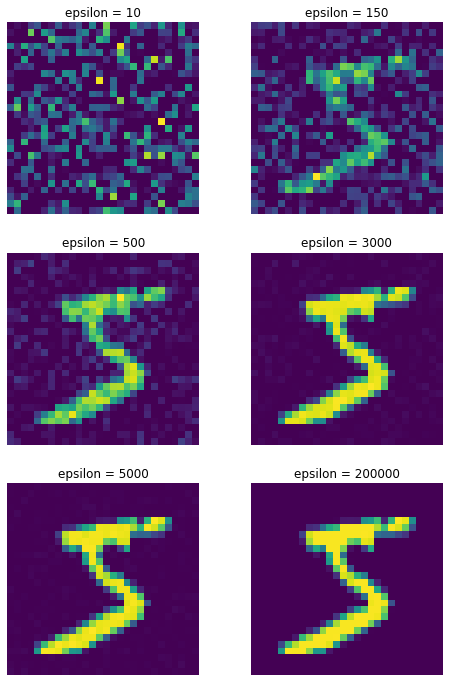
\includegraphics[width=0.5\textwidth]{figures/epsilons.png}
      \caption{Effects of Gaussian Noise for different values of $\epsilon$}
\end{figure}

Here we see the results of the neural networks trained and evaluated on the re-clustered labels. Notice that the images become very obviously distinguishable at around $\epsilon = 500$. We add noise by sampling from a gaussian distribution, using the gaussian mechanism for differential privacy with the specified $\epsilon$ parameters.
\subsection{Invariant Information Clustering with Gaussian-noised Data}
After following through several methods initially and consistently achieving low accuracy scores, we turned to state of the art methods. 

The noising of the labels turned out to be more complicated than anticipated, so we chose an elegant solution to this problem that uses unsupervised clustering to generate labels for the data in a private way. This solution was replicated from a paper (2) that uses this unsupervised method of generating synthetic labels on the MNIST dataset. This paper, however, did not add noise to the training data, so we used input perturbation to develop our own noisy input data. We then took that noisy data and used the paper's model to generate both noisy labels and a neural network classifier. 

To generate the noisy input data, we first took the 28x28 image and normalized the pixel values so that the L2 norm of all the pixel values is 1. We then added Gaussian noise using the Gaussian mechanism to the data, with parameter values of sensitivity = 1, $\epsilon \in \{150, 2000, 3000, 5000, 200000\}$, and $\delta = 1/(28\cdot 28)^2$ (i.e., $1/n^2$). The model then builds a neural network classifier from the noisy input data and the labels. The model works by taking an input dataset and then applying an image transformations like rotation and cropping- this is what makes the model invariant. At this point, both datasets are run through an unsupervised CNN and then a fully connected neural network to learn the natural clusters within the data. Because these labels are being generated without knowing the true labels, they are private. 



\section{Description of Results}
We present the results of the three different methods of classification discussed in the technical description section. We only show the results using $\epsilon = 2000$, as the other models showed even worse performance. 
\subsection{Differentially Private Neural Networks}
The first method discussed was to experiment with differing depths and architecture's of neural networks applied to learning from differentially private image sets. Figure 2 displays the results from three different experiments, a non differentially private reference model set (Images 2d, 2e), using the noisy image and noisy label(Images 2a,2b), and re clustering the noisy images and then using those as labels to training a CNN (Images 2c,2d).  
\newpage
\begin{figure}
    \centering
    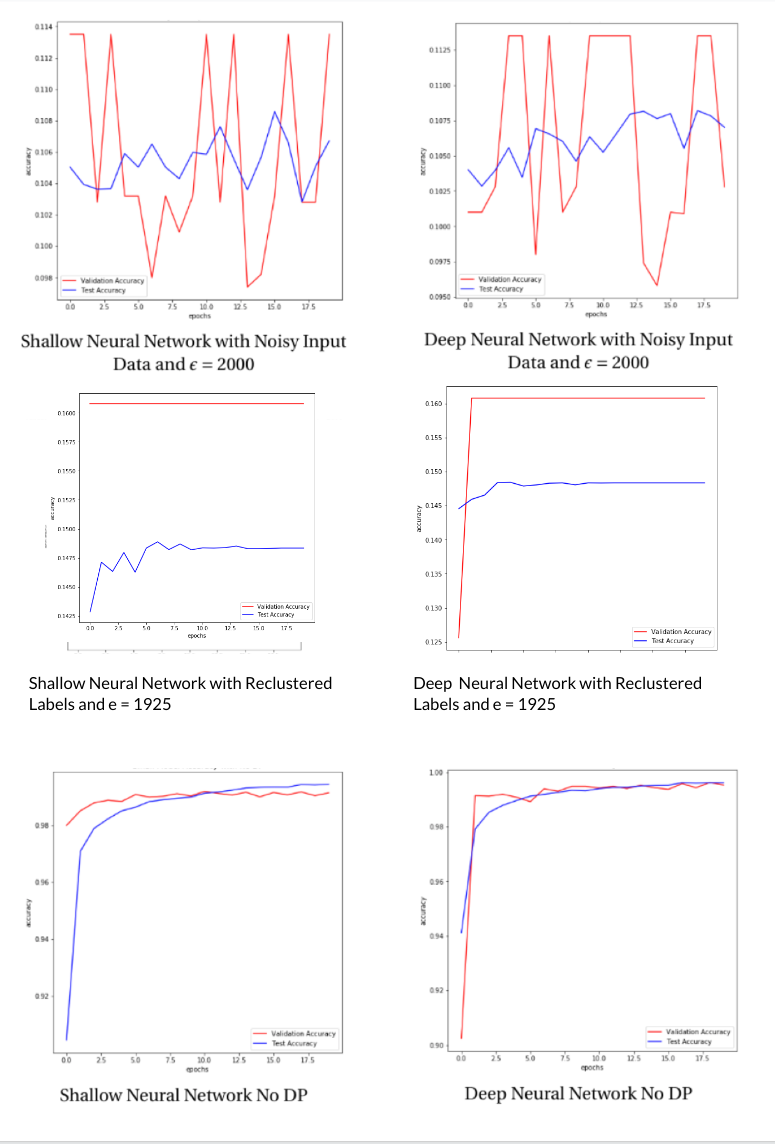
\includegraphics[scale = 0.6]{new_fig.png}
    \label{fig:my_label}
    \caption{Gaussian Noise Injection, Reclustering and Standard Neural Network Performance with MNIST}
\end{figure}
We see that both networks do not perform well on the Noisy Image,Label pairs. The training accuracy does not show a clear increase, and the testing accuracy indicates that the model is classifying according to the class balance, as there are only 10 classes. From these results, we do not recommend using the vanilla local differential privacy approach to the MNIST problem, as the noise is simply too damaging to the performance of the neural networks, even with a very high $\epsilon$.\\\\
Further, in images 2c and 2d, we see that the models are  improved when the clustered image labels are used as opposed to the noisy labels. The improvement is slight, but still only occurs with an unrealistic value of $\epsilon$. However, this is a distinct improvement of over the first implementation, as there is a higher accuracy and the true labels never need to be used, leading to a lower privacy cost. 

The oscillating learning rate of the two models is interesting and cannot readily be explained. 

See section 0.4.1.1 and Image 3 for a description of the Kmeans clustering results. 


\subsubsection{KMeans}


As we can see in the image below, using the re-clustered labels as labels for the noised images marginally increases the performance of the neural networks. Figure 3 shows the performance of the KMeans clustering algorithm on the noisy image data. It is clear that the results are not great; however, the accuracy is still better than if we had just noised the original labels.


\begin{figure}[H]
  \centering
    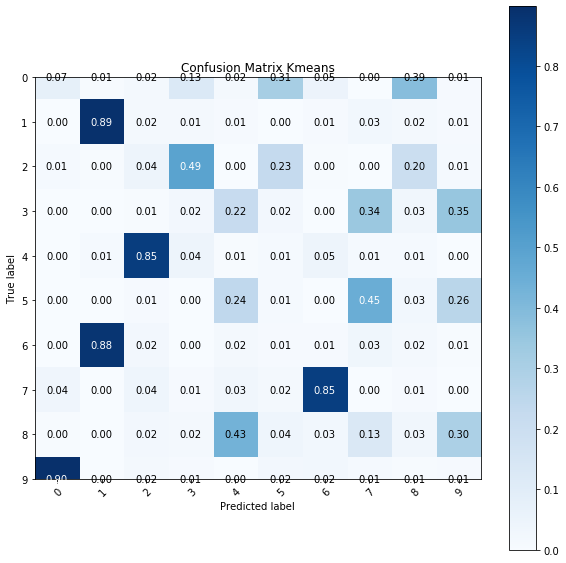
\includegraphics[width=0.5\textwidth]{figures/confusion_matrix.png}
      \caption{Confusion Matrix for KMeans Clustering}
\end{figure}


\subsection{Invariant Information Clustering with Gaussian-noised Data}
As expected, the model trained on the raw data performs extremely well and achieves a classification error of under 10 percent, with the loss dropping down to below -2.5.

As noise is added to the images, the performance immediately and dramatically decreases. Initially, with an epsilon of 150 which seemed reasonable (see figure 1) we can see that the loss bottoms out at -0.7 and the classification error never drops below 0.89. This is the proportion of examples in the plurality class .

To summarize, we see that with an epsilon of 150 and 2000, the model is just picking up the plurality class. An epsilon of 3000 does better; however, still not as good as the model trained on the raw data. An epsilon value of 5000 surprisingly performs worse than an epsilon value of 3000, and this could be just due to the random initializations. An epsilon value of 200000 performs well; however, this case effectively adds no noise to the data. We found the magnitude of epsilon that we had to hit just to see improvements in our results to be very surprising and disappointing. 







\begin{figure}[H]
  \centering
  \begin{minipage}{0.45\textwidth}
    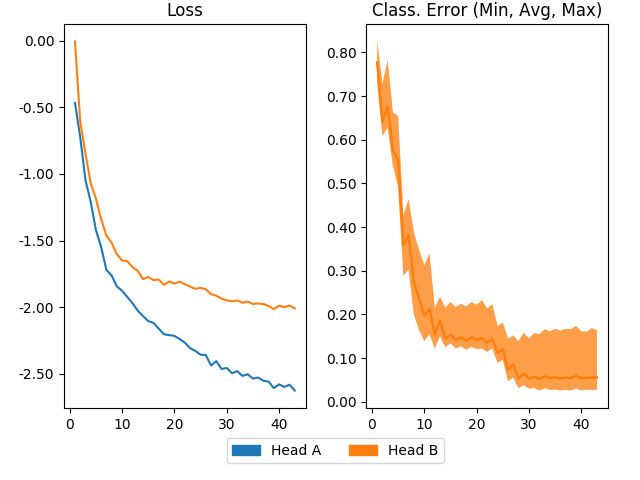
\includegraphics[width=\textwidth]{figures/normal.png}
    \centering
    IIC Model with raw data.
  \end{minipage}%
  \hspace{0.09\textwidth}
  \begin{minipage}{0.45\textwidth}
    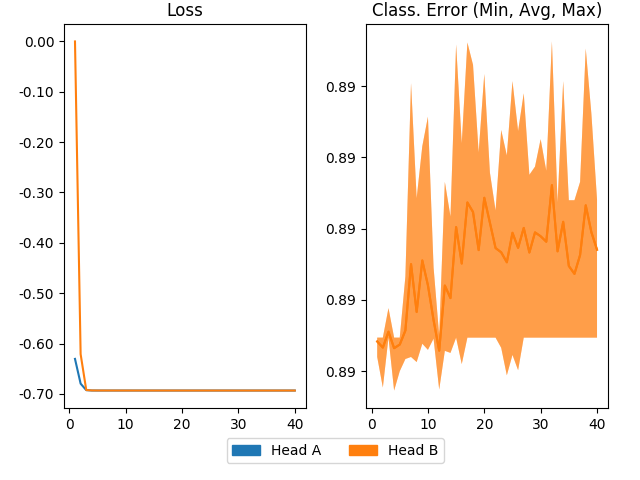
\includegraphics[width=\textwidth]{figures/epsilon-150.png}
    \centering
    IIC Model with $\epsilon=150$.
  \end{minipage}%
  \\[2em]
    \begin{minipage}{0.45\textwidth}
    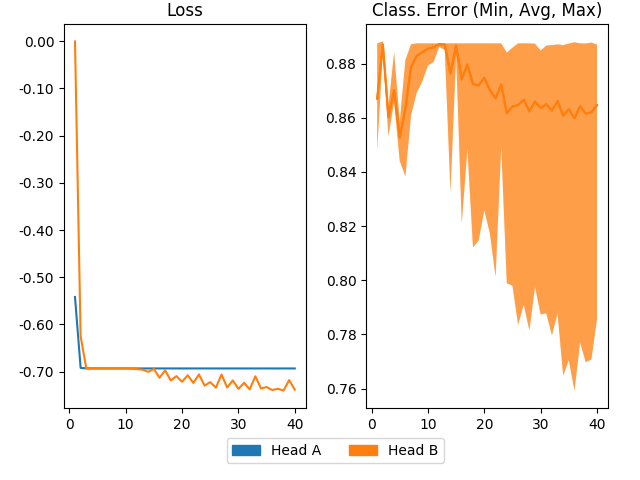
\includegraphics[width=\textwidth]{figures/epsilon-2000.png}
    \centering
    IIC Model with $\epsilon=2000$.
  \end{minipage}%
  \hspace{0.09\textwidth}
  \begin{minipage}{0.45\textwidth}
    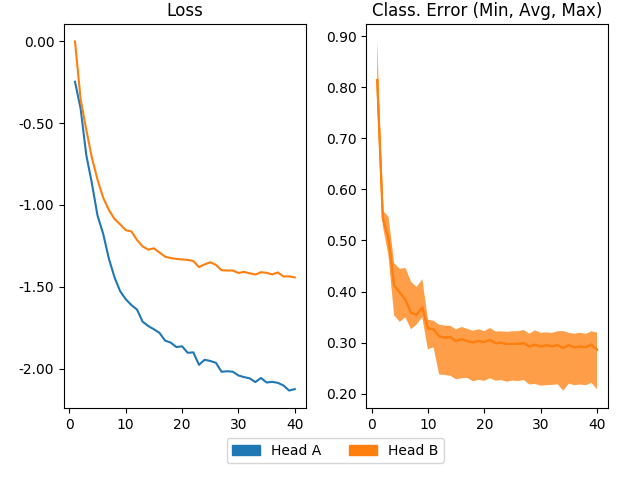
\includegraphics[width=\textwidth]{figures/epsilon-3000.png}
    \centering
    IIC Model with $\epsilon=3000$.
  \end{minipage}%
  \\[2em]
    \begin{minipage}{0.45\textwidth}
    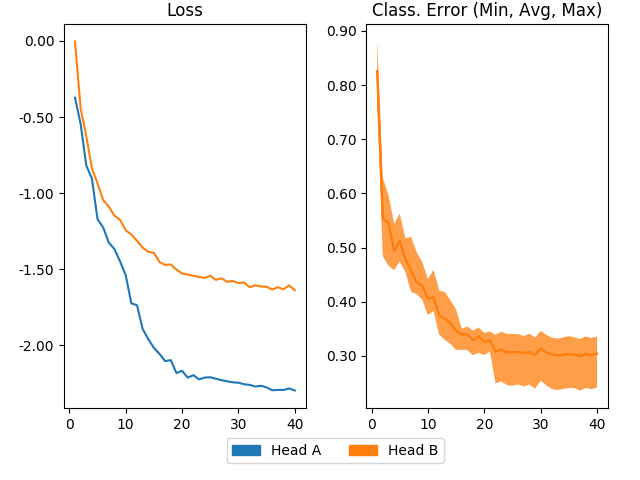
\includegraphics[width=\textwidth]{figures/epsilon-5000.png}
    \centering
    IIC Model with $\epsilon=5000$.
  \end{minipage}%
  \hspace{0.09\textwidth}
  \begin{minipage}{0.45\textwidth}
    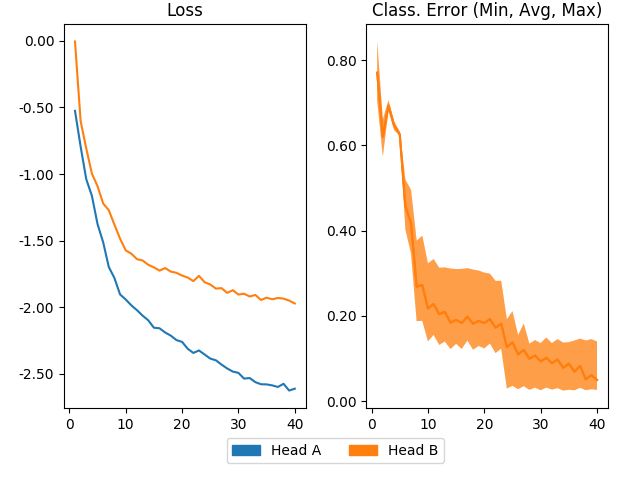
\includegraphics[width=\textwidth]{figures/epsilon-200000.png}
    \centering
    IIC Model with $\epsilon=200000$.
  \end{minipage}%
  \\[2em]
  \caption{Training loss and performance of IIC models with varying privacy costs. Note that the vertical axes are not consistent between subplots, so heights cannot be compared directly. We see that the model using the raw data performs extremely well, achieving an error rate of less than 10 percent. However, any models which are differentially private suffer greatly when it comes to performance, until $\epsilon$ becomes extraordinarily large.}
\end{figure}



\section{Implementation}
Our implementation is available at \url{https://github.com/maxfieldEland/dp_nueral_nets}. For the IIC model, a diff of our modifications to the original implementation. For a generation of the results, see the driver.py file, which will read in MNIST data, build models and plot presented graphs accordingly.  (\url{https://github.com/astirn/IIC}) can be found in \texttt{iic/dp-diff.txt}.



\section{Sources}
1. Tremblay, J., Prakash, A., Acuna, D., Brophy, M., Jampani, V., Anil, C., … Birchfield, S. (2018). Training Deep Networks with Synthetic Data: Bridging the Reality Gap by Domain Randomization. 2018 IEEE/CVF Conference on Computer Vision and Pattern Recognition Workshops (CVPRW). doi: 10.1109/cvprw.2018.00143

2. Ji, X., Henriques, J. F., & Vedaldi, A. (2019). Invariant information clustering for unsupervised image classification and segmentation. In Proceedings of the IEEE International Conference on Computer Vision (pp. 9865-9874).

% Questions to Answer
% Is the paper answering the “right” question?
% Does it make reasonable assumptions?
% How novel is the solution?
% Is the solution technically sound?
% Is the solution difficult or easy?
% How well is the solution evaluated?
% Expected impact (hard to guess)
% Writing level: is the paper clearly written? Is it self-contained?
\end{document}